\documentclass{beamer}

\mode<presentation> {
  %\usetheme{Warsaw}
  \usetheme{PaloAlto}
  \setbeamercovered{transparent}
}

\usepackage{listings}
\usepackage{ucs}
\usepackage[utf8x]{inputenc}
\usepackage[czech]{babel}
\usepackage{palatino}
\usepackage{graphicx}
\usepackage{caption}
\usepackage{subcaption}
\usepackage{wrapfig}
\usepackage{epsfig}

\usepackage{tikz}
\usetikzlibrary{shapes,arrows}

\usepackage{float}

%makra
\def\cmd#1{{\tt #1}}	% sazba příkazu
\def\fnm#1{{\sf #1}}    % sazba jména souboru
\def\emp#1{{\bf #1}}    % sazba zvýraznění textu


\addtobeamertemplate{navigation symbols}{}{%
    \usebeamerfont{footline}%
    \usebeamercolor[fg]{footline}%
    \hspace{1em}%
    \insertframenumber/\inserttotalframenumber
}




\usepackage{tikz}
\usetikzlibrary{arrows,shapes,positioning,shadows,trees}

\tikzset{
    %Define standard arrow tip
    >=stealth',
    %Define style for boxes
    punkt/.style={
           rectangle,
           rounded corners,
           draw=black, very thick,
           text width=6.5em,
           minimum height=2em,
           text centered},
    % Define arrow style
    pil/.style={
           ->,
           thick,
           shorten <=2pt,
           shorten >=2pt,}
}


\title{Hackathon 2017 - Robot NAO}
\author{Tým - Markers}
\date{3.3.2017 -- 5.3.2017}

\begin{document}


\begin{frame}
  \titlepage
\end{frame}


\section{Zadání}
\begin{frame}
\frametitle{Zadání}  
	\begin{itemize}
		\item{Pokusit se o inventarizaci skladu pomocí robota NAO}
		\item{Cesta po markerech a skenování QR kódů}
		
		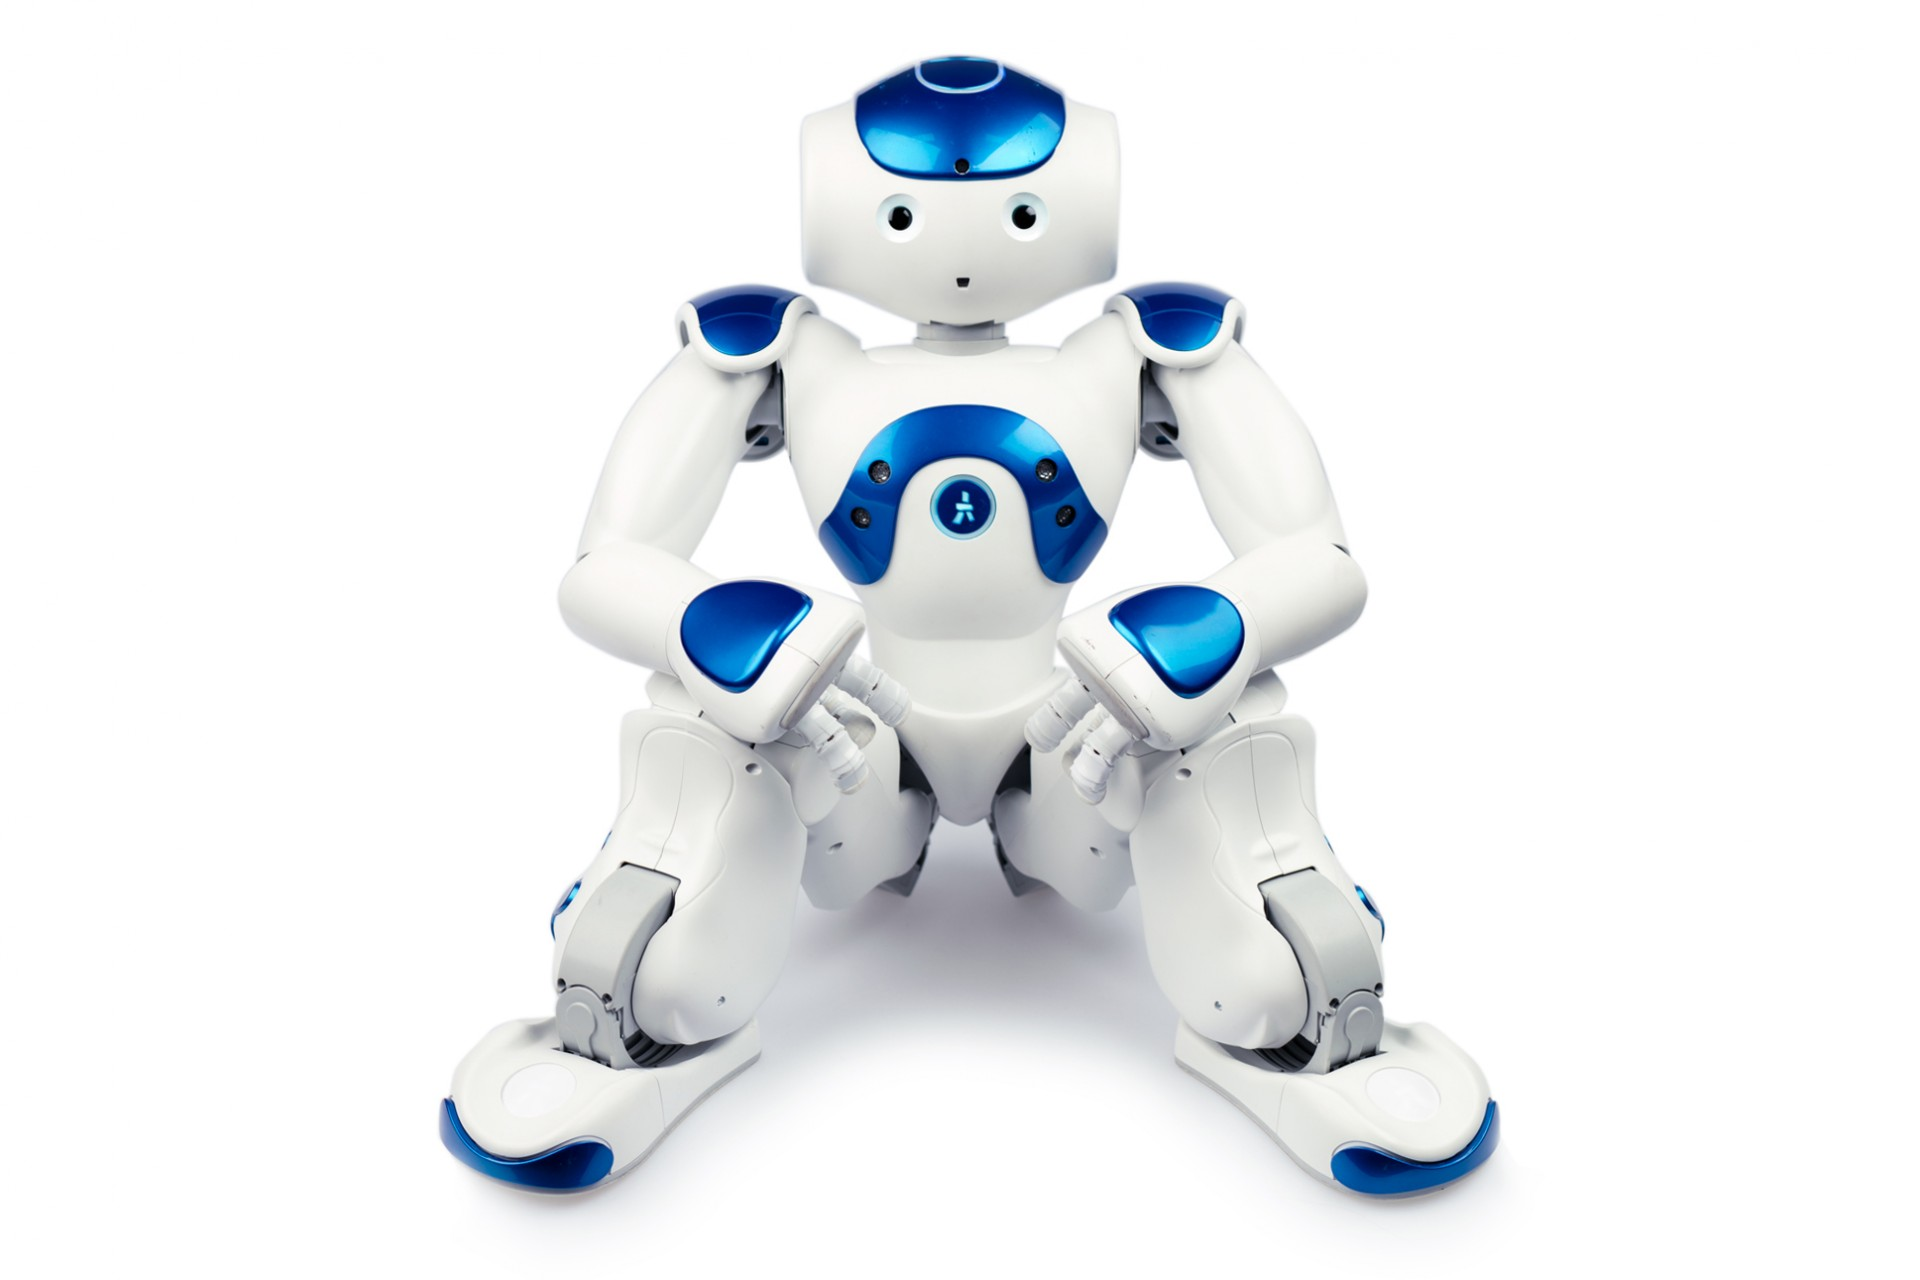
\includegraphics[width=8cm]{img/nao.jpg}
		
	\end{itemize}
 
\end{frame}

\section{Zpracování}
\begin{frame}
\frametitle{Zpracování -- Počátek}  
	\textbf{Vývoj v Javě}
	\begin{itemize}		
	
		\item{Zprovoznění čtení textu -- Hello World}
		\item{Základní polohy: stoj, poklek a sed}
		\item{Různé pohyby končetin a hlavy}			
				
	\end{itemize}
	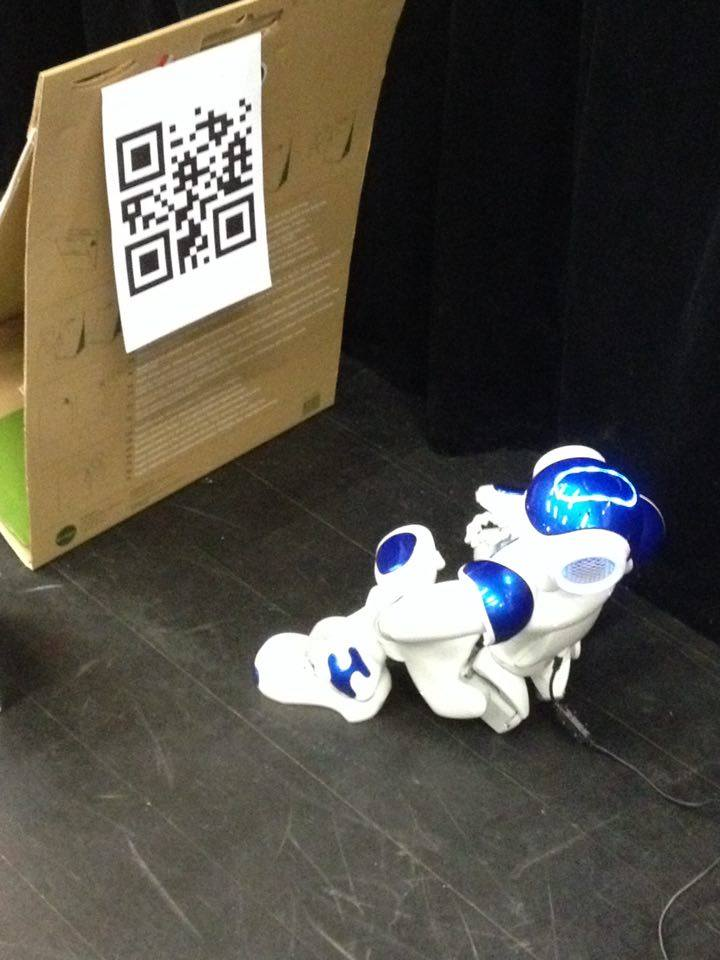
\includegraphics[width=4cm]{img/nao_kouka.jpg}

 
\end{frame}

\begin{frame}
\frametitle{Zpracování -- Další krůčky}  
	\begin{itemize}
		\item{Zprovoznění předních kamer.}
		\item{Knihovna na zpracování QR kódů.}						
		\item{Počátek trackování -- červený míček.}
			\begin{itemize}
				\item{Nejprve Python (točení hlavy, poté následování).}
				\item{Posléze nasazení do Javy a pokusy o zdolání cesty po červených kruzích.}
			\end{itemize}
	\item{Problém lesknutí obrázků na zemi.}
	\item{Synchronizace rozhlížení a skenování.}	
	\end{itemize}
 
\end{frame}

\begin{frame}
\frametitle{Zpracování -- Očima Romea I}  
	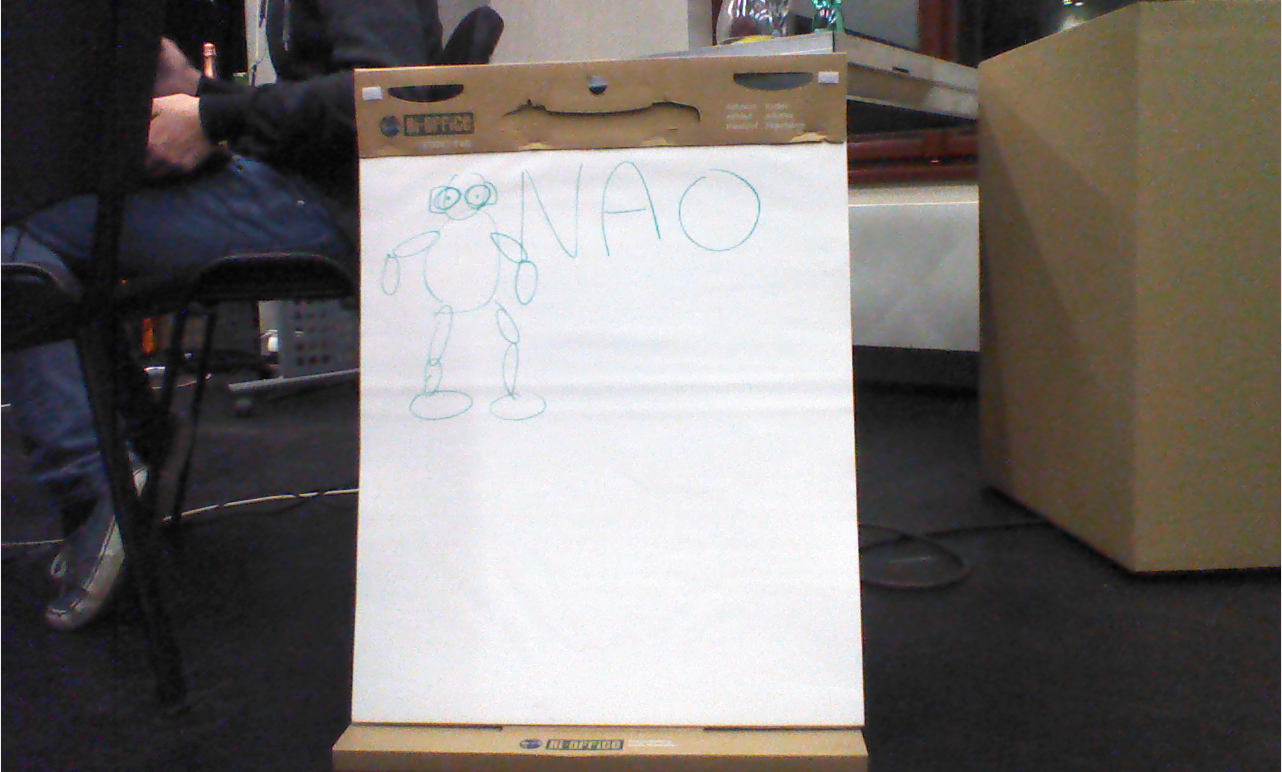
\includegraphics[width=\textwidth]{img/nao_jeho_pohled.png}	 
\end{frame}

\begin{frame}
\frametitle{Zpracování -- Očima Romea II}  
	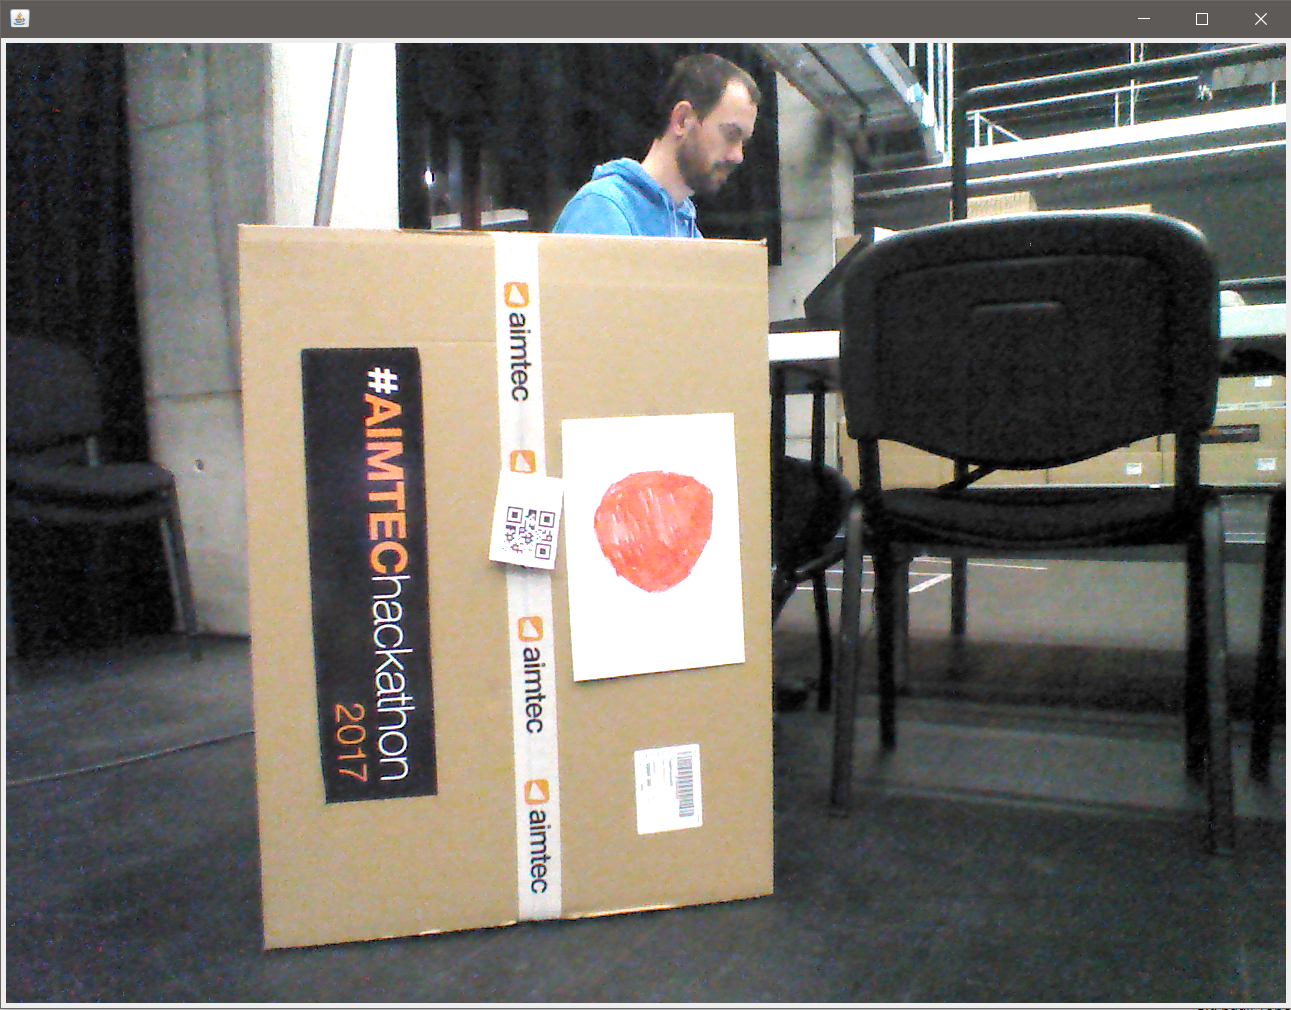
\includegraphics[width=\textwidth]{img/nao_jeho_pohled2.png}	 
\end{frame}

\begin{frame}
\frametitle{Zpracování -- Očima Romea III}  
	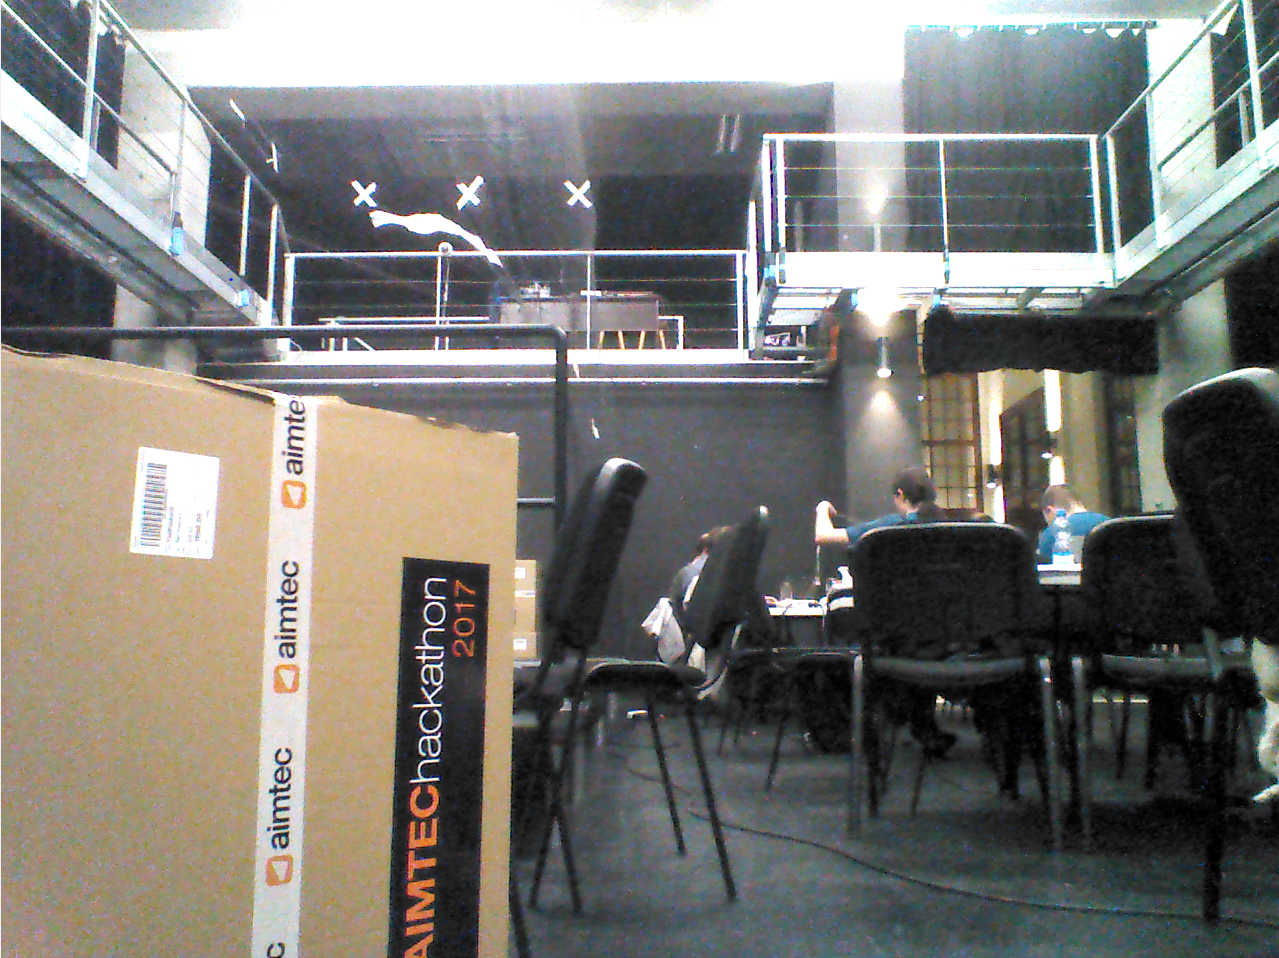
\includegraphics[width=\textwidth]{img/nao_jeho_pohled3.png}	 
\end{frame}


\section{Závěr}
\begin{frame}
\frametitle{Závěr} 
	\begin{itemize}
		\item{Zkušenosti}
		\item{Vzpoura robotů}
	\end{itemize}
	Ukázky kódu:
	\small{\url{https://github.com/aimtechackathon2017/markers}}
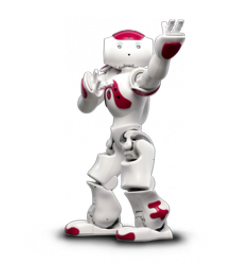
\includegraphics[width=5cm]{img/nao_ukazuje.png}	


\end{frame}

\end{document}






















